Masukkan code berikut untuk test navigator pada menu  Panduan:
\begin{verbatim}
  panduan = browser.get('https://tokoperhutani.com/panduan')
\end{verbatim}

Hasilnya  di Mozilla Akan mucul seperti ini :
\begin{figure}[h]
\centering
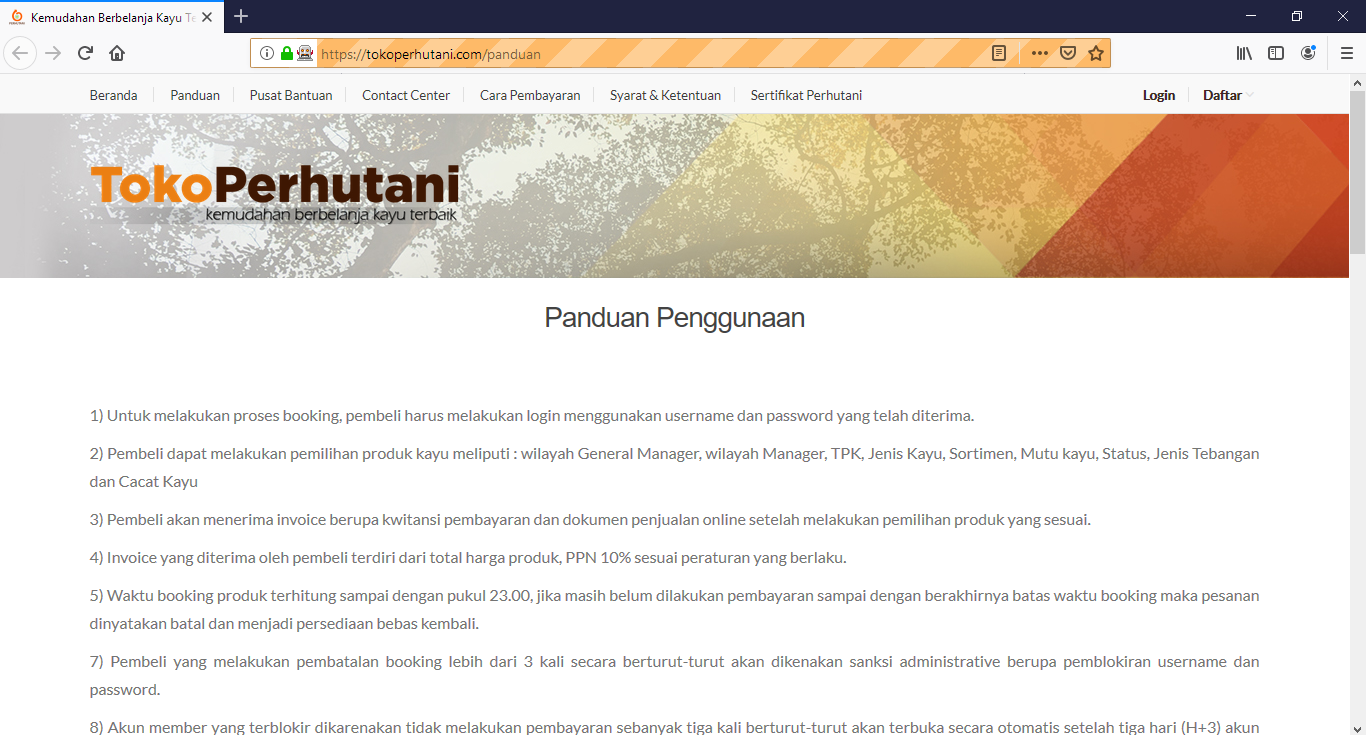
\includegraphics[scale=0.3]{figures/1hasil.PNG}
\caption{Navigator Pada Panduan}
\end{figure}

Masukkan code berikut untuk test navigator pada menu  Pusat bantuan:
\begin{verbatim}
  pusatbantuan = browser.get('https://tokoperhutani.com/faqs')
\end{verbatim}

Hasilnya  di Mozilla Akan mucul seperti ini :
\begin{figure}[h]
\centering
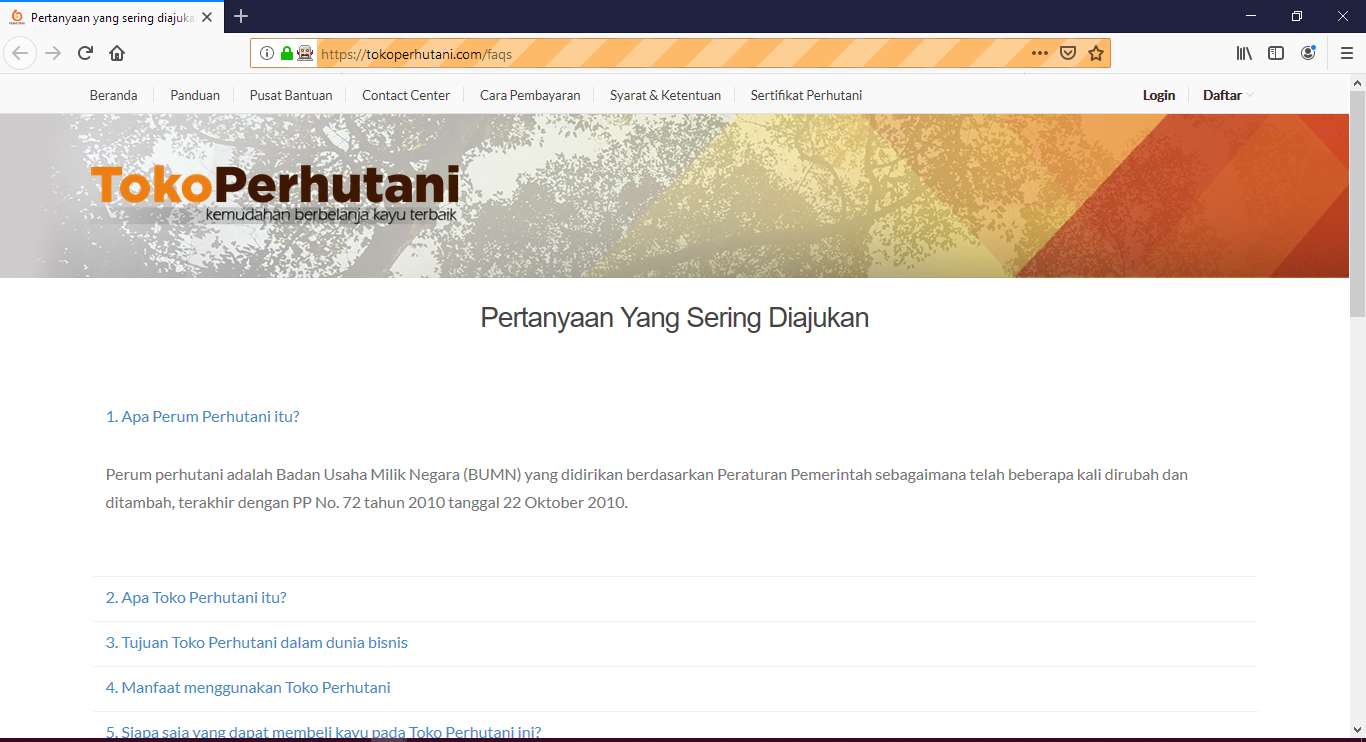
\includegraphics[scale=0.3]{figures/2hasil.PNG}
\caption{Navigator Pada Pusat Bantuan}
\end{figure}

Masukkan code berikut untuk test navigator pada menu  Alamat kantor:
\begin{verbatim}
  alamatkantor = browser.get('https://tokoperhutani.com/article/detil/alamat-kantor')
\end{verbatim}

Hasilnya  di Mozilla Akan mucul seperti ini :
\begin{figure}[h]
\centering
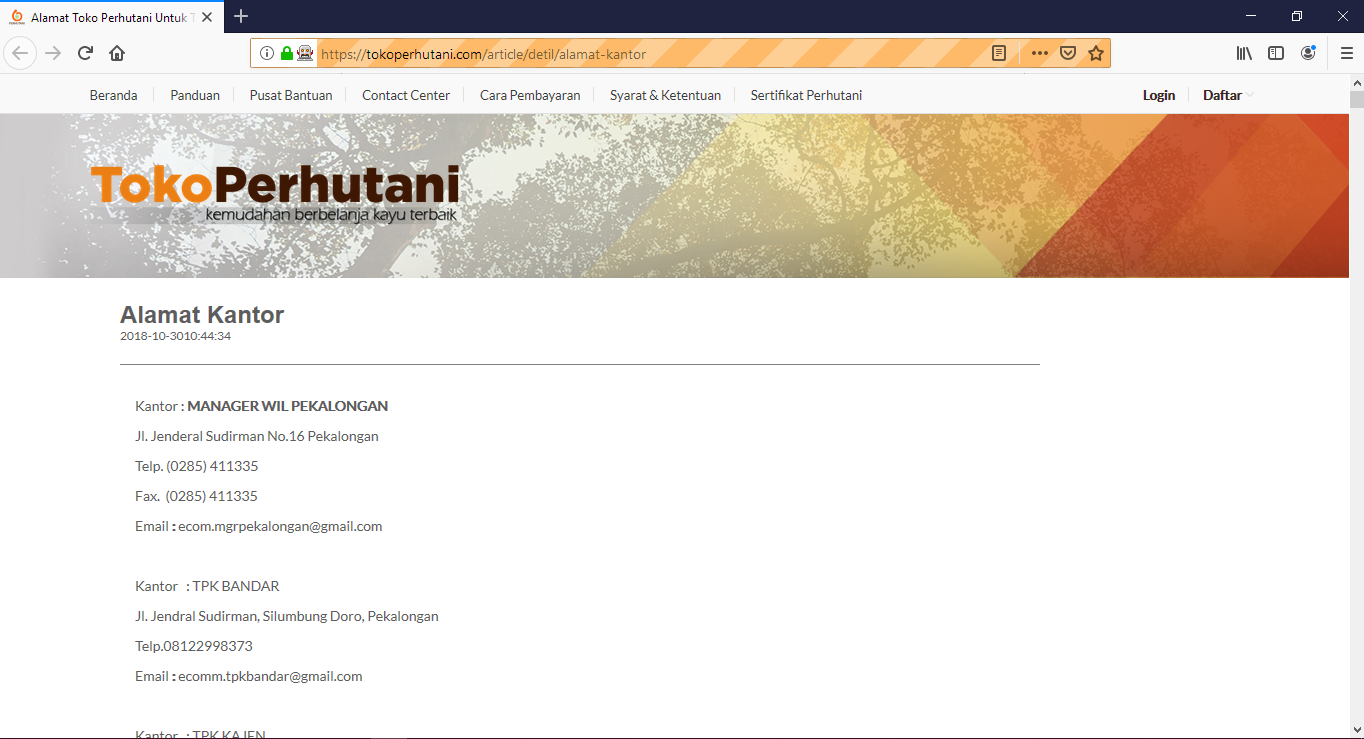
\includegraphics[scale=0.3]{figures/3hasil.PNG}
\caption{Navigator Pada Alamat Kantor}
\end{figure}

